\documentclass[a4paper,10pt,twoside]{article}

\usepackage{revista-heuristica}

\titlerevista[T\'itulo corto del art\'iculo]{Análisis Factorial Múltiple (AFM)}
\authorrevista[1][García, K.]{García C. Kevin}
\institucionmail[1][Escuela de Estadistica]{Universidad del Valle, Facultad de Ingenier\'ia}{pedro.perez@correounivalle.edu.co}
\authorrevista[2][Buitron, N.]{Buitron. Natalia}
\institucionmail[2][Universidad del Valle, Facultad de Ingenier\'ia]{Escueal de Estad\'istica}{pablo.gimenez@correounivalle.edu.co}
\authorrevista[3][Soto, A.]{Soto. Alejandro}
\institucionmail[3][Universidad del Valle, Facultad de Ingenier\'ia]{Escueal de Estad\'istica}{pablo.gimenez@correounivalle.edu.co}
\authorrevista[4][Vargas, A.]{Vargas. Alejandro}
\institucionmail[4][Universidad del Valle, Facultad de Ingenier\'ia]{Escueal de Estad\'istica}{pablo.gimenez@correounivalle.edu.co}

\nombrerevista{Heur\'istica}
\issnrevista{2422-5177}
\volumenrevista{18}
\mesrevista{Mayo}
\aniorevista{2015}
\numerorevista{1}

\setcounter{page}{1}

\sethdrevista
\makeatletter
%con esto, definimos el comando \blfootnote{texto de pie de pagina} que genera un pie de pagina sin numeracion.
\def\blfootnote{\xdef\@thefnmark{}\@footnotetext}
\makeatother

\begin{document}

\label{PrimeraPagina}
\thispagestyle{fancy}
\twocolumn[
    \begin{@twocolumnfalse}
  	\maketitlerevista
  	\thispagestyle{empty}  
  	\vfill
  	\renewcommand\abstractname{}
  	\begin{abstract}
      
      \hrulefill
      
      \textbf{Abstract:} The following instructions set the guidelines for the preparation of articles for the Heurística magazine of School of Statistics at the Universidad del Valle. Articles may be written in Spanish or English, but must have an abstract in both languages. Authors can use this document as a template to compose your article. Otherwise, this document can be used as an instruction guide. The maximum number of pages is 12. The summary should present the objectives and scope of work, as well as its main results and conclusions. The abstract must be faithful English version of the summary. Both the abstract and the Resumen should contain no more than 150 words to avoid affecting the final layout of the magazine.
      
      \keywordsrevista{The same keywords in Spanish}
    \end{abstract}
    \vspace{-3\baselineskip}
    \begin{abstract}
    
      \textbf{Resumen:} Las siguientes instrucciones establecen las pautas para la preparación de artículos para la Revista Heurística de la Escuela de Estadística de la Universidad del Valle. Los artículos pueden ser escritos en español o en inglés, pero deben tener un resumen en ambos idiomas. Los autores pueden hacer uso de este documento como una plantilla para componer su artículo. Caso contrario, este documento puede ser utilizado como una guía de instrucciones. El número máximo de páginas será 12. El Resumen debe presentar los objetivos y el alcance del trabajo, al igual que sus principales resultados y conclusiones. El abstract debe ser la versión fiel en inglés del resumen. Tanto el abstract como el resumen NO DEBEN contener más de 150 palabras para no afectar la diagramación final de la revista.
      
      \palabrasclavesrevista{Se puede incluir hasta 7 palabras o frases clave a continuación del resumen, cada una con un máximo de 3 palabras por frase. Las mismas palabras clave deben reproducirse en ingles y estar ordenadas en orden alfabético.}
      
       \hrulefill
    \end{abstract}  
    
    \end{@twocolumnfalse} 
  ]

  \clearpage

  \section{Introducci\'on}
  
\blfootnote{\footnotesize Artículo recibido el XX; revisado XX. (Escriba la fecha en que presentó su documento para su revisión). 

Esta sección puede ser utilizada para colocar información adicional de los autores. Evite escribir fórmulas largas con subíndices en el título; fórmulas cortas que identifican los elementos están bien (por ejemplo, ``Nd-Fe-B''). No escriba ``(invitado)'' en el título. se prefieren en el campo de autor Los nombres completos de los autores.

\begin{description}
  \item[*] Estudiante Msc. en Ingeniería Industrial, Universidad del Valle. Ingeniera Industrial, Universidad del Valle.
  \item[**] Estudiante Msc. en Ingeniería Industrial, Universidad del Valle. Ingeniera Industrial, Universidad del Valle. 
  \item[***] Msc. en Ingeniería Industrial, Universidad del Valle. Especialista en Logística, Universidad del Valle. Ingeniero Industrial, Universidad del Valle . Profesor de planta de la Universidad del Valle desde el 2007.
\end{description}

Autor para correspondencia: Dirección de Autor FA correos electrónicos, teléfono y dirección institucional.

}
  
  La Revista Heurística es una publicación científica y tecnológica de la Escuela de Estadística de la Facultad de Ingeniería de la Universidad del Valle, cuyo objetivo es el de publicar artículos en cualquiera de las áreas de estadística, investigación de operaciones, sistémica y áreas relacionadas con las anteriores. 

  Los artículos pueden estar escritos en español o en inglés y pueden enmarcarse dentro de la clasificación de artículos dada por Colciencias:

  \textbf{Artículos de Investigación científica} o tecnológica: Presentan resultados originales de investigación.

  \textbf{Artículos de reflexión:} Presentan resultados de investigación sobre un tema específico  desde la perspectiva analítica interpretativa o critica de los autores, recurriendo a fuentes bibliográficas originales.

 \textbf{Artículos de revisión:} Presentan el resultado de una revisión analítica de la literatura sobre un tema especifico, sistematizando o integrando los resultados de investigaciones ya publicadas con el fin de dar cuenta del avance y las tendencias de desarrollo de ese tema. Incluyen una cuidadosa y amplia revisión bibliográfica.

  Se consideran igualmente las siguientes clasificaciones de artículos y notas cortas:

  \textbf{Casos y Notas técnicas:} Se publican aquí casos de estudio que no puedan enmarcarse dentro de las categorías anteriores. Las notas técnicas, por su parte, son informes cortos sobre aspectos específicos cuya longitud y alcance no clasifica como artículo completo.

  \textbf{Ensayo:} Consiste en una reflexión filosófica, pedagógica, histórica o literaria o una combinación de éstas, en la cual se trata uno o más problemas de los múltiples que pueden caber en una escuela como la estadística. Son bienvenidas las reflexiones críticas que liguen el quehacer universitario con las realidades sociales de nuestro país, región o departamento.

  \textbf{Comentarios de libros:} Se publican aquí comentarios de libros recientemente publicados, relacionados con las áreas temáticas de la revista.

  La edición de la revista es anual. Los artículos deben ser originales y no deben encontrarse bajo evaluación en otras revistas.

Este documento es una plantilla para LaTeX.  Por favor, no coloque ningún número consecutivo, encabezado / pie de página en el documento presentado.

Puede escribir sobre las secciones de éste documento o cortar y pegar de otro documento. se recomienda el uso del programa TeXMaker, para la edición de sus artículos o cualquier editor de textos LaTeX que sea de su preferencia.

%a la izquierda de la barra de herramientas de formato, en la parte superior de la ventana de Word (por ejemplo, el estilo en este punto del documento es “Texto”). Resalte una sección que usted quiera designar con un cierto estilo, y luego seleccione el nombre apropiado en el menú de estilo. El estilo ajustará los tipos de letra y espaciado de línea. No cambie los tamaños de fuente o espaciado de renglones para ajustar el texto a un número limitado de páginas. Utilice cursiva o negrita para dar énfasis a un texto, no subrayado.

  \section{PROCEDIMIENTO PARA LA PRESENTACIÓN DEL ARTÍCULO}
  
  \subsection{Etapa de Revisión}
  
Por favor, utilice este documento como una “plantilla” para preparar el manuscrito. Para las pautas de presentación, siga las instrucciones emitidas por el sistema del sitio web de la revista de la EPN.

La presentación inicial debe tomar en cuenta todas las indicaciones que se presentan en esta plantilla, para de esta manera tener una buena estimación de la longitud del artículo a publicarse. Además, de esta manera el esfuerzo necesario para la presentación final del manuscrito será mínimo.
  
  Los manuscritos deben ser enviados al Editor Jefe de la revista en forma electrónica al correo: \url{revista.heuristica@correounivalle.edu.co}. 
  
  La estructura general de los artículos debe ser la siguiente:
  
  \begin{description}
  \item[Contenido:] El articulo no debería exceder las 12 páginas, incluyendo tablas, figuras, apéndices y referencias bibliográficas. 
  \item[T\'itulo:] El titulo del manuscrito debe reflejar sin ambigüedades y en forma concisa el contendido y alcance del trabajo. Deben evitarse títulos de más de 20 palabras.
  \item[Autores:] Se debe incluir el primer nombre del autor,  la inicial de su segundo nombre si aplica, y el primer apellido completo. Para cada autor se debe indicar la afiliación en el apartado \emph{blfootnote} que se encuentra iniciando el documento, allí se debe indicar la facultad, escuela, institución, empresa u organización a la que pertenezca el autor, incluyendo su dirección y su correo electrónico.
   \end{description}
  
  \subsection{Etapa Final}
  
Los autores deben trabajar activamente con los márgenes de tiempo solicitados. Los documentos de la revista serán marcados con los datos del registro de la revista y paginados para su inclusión en la edición final. Se pedirá una última revisión por parte del autor de cada artículo, antes de dar por finalizada la edición y posterior lanzamiento de la revista.

%Formulario Copyright

%La Revista Heurística pondrá en marcha un sistema de transferencia electrónica de derechos de autor en su momento. Por favor, “no” enviar formularios de derecho de autor por correo o fax. Más información sobre este tema estará disponible en el sitio web de la revista.

\section{Edición}
  
  \subsection{Texto principal}
  
  Generalmente los artículos de investigación científica y tecnológica deben contener las siguientes secciones o sus equivalentes:
  
  \begin{enumerate}
   \item Introducción
   \item Metodología
   \item Resultados y discusión
   \item Conclusiones
  \end{enumerate}
  
  Cada una de estas secciones puede contener subsecciones, las cuales deben numerarse de acuerdo con el número de la subsección. Se recomienda, sin embargo, no sobrepasar de dos niveles de numeración.
   
  El texto principal puede contener un Apéndice, el cual comprende elementos no esenciales para la lectura del texto principal, pero que podrían aclarar aspectos importantes a lectores que lo requieran, como por ejemplo demostraciones de teoremas, códigos de programa, aclaraciones, tablas secundarias, etc. Igualmente el texto principal puede contener una sección de agradecimientos, inmediatamente después de las conclusiones (o de los apéndices si existen). La posición relativa de estos elementos es la siguiente: Conclusiones, Apéndice (si lo hay), Agradecimientos (Si los hay) y Referencias Bibliográficas.
  
  \subsection{Figuras}
  
\begin{figure}%[h!] %h! sirve para dejar la imagen en el sitio donde la estoy colocando h=here%
	\begin{center}
	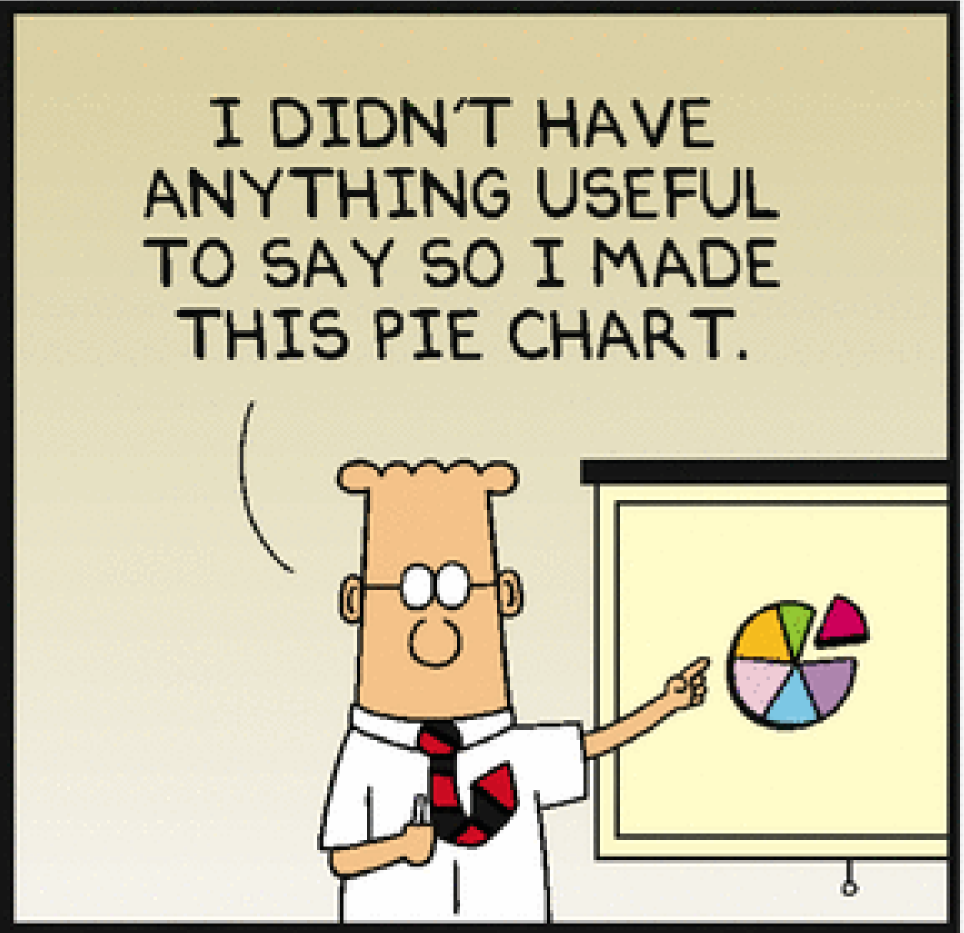
\includegraphics[width=7cm,keepaspectratio=true]{./imagenes/pie}
	% pie.png: 0x0 pixel, 300dpi, 0.00x0.00 cm, bb=
	\end{center}
	\caption{``Como no ten\'ia nada \'util para decir, constru\'i esta torta'' \citep{Adams2009} \citep{Olaya2015}}
	\label{fig1}
\end{figure}   
  
  Todas las figuras deben ser incorporadas en el documento. Al incluir la imagen, asegúrese de insertar la dirección correcta y ubicar las imágenes en la carpeta \emph{imagenes} tal y como se encuentra en éste documento. En lo posible, utilice imágenes en formato pdf o png\footnote{Recuerde que si las imágenes se encuentran en formato pdf o png, es suficiente con utilizar el comando de compilación pdflatex, si se desea utilizar figuras en formato eps y ps se debe utilizar el comando de compilación latex, luego generar el pdf con el comando pstopdf.} de alta calidad (preferiblemente a 300ppp).
  
  El argumento \emph{width=6 cm} garantiza un ancho de la imagen de 6cm; también se puede utilizar el argumento \emph{scale=0.5} el cual disminuye el tamaño de la imagen al 50\% de forma tal que se pueden modificar estos valores hasta conseguir el resultado esperado en el pdf resultante como se puede observar en la figura \ref{fig1}. 
  
  El argumento \emph{keepaspectratio=true} permite que la imagen no se distorsione al modificar su tamaño. El título de las figuras debe estar en la parte inferior correctamente numerada y en caso de que las figuras no sean producto del autor se debe indicar la fuente.
  
  En el caso de las imágenes grandes que no puedan ser reducidas debido a información que debe ser legible se debe utilizar el entorno \textbf{figure*} tal y como se aprecia en la figura \ref{fig2}.
  
\begin{figure*}
\centering
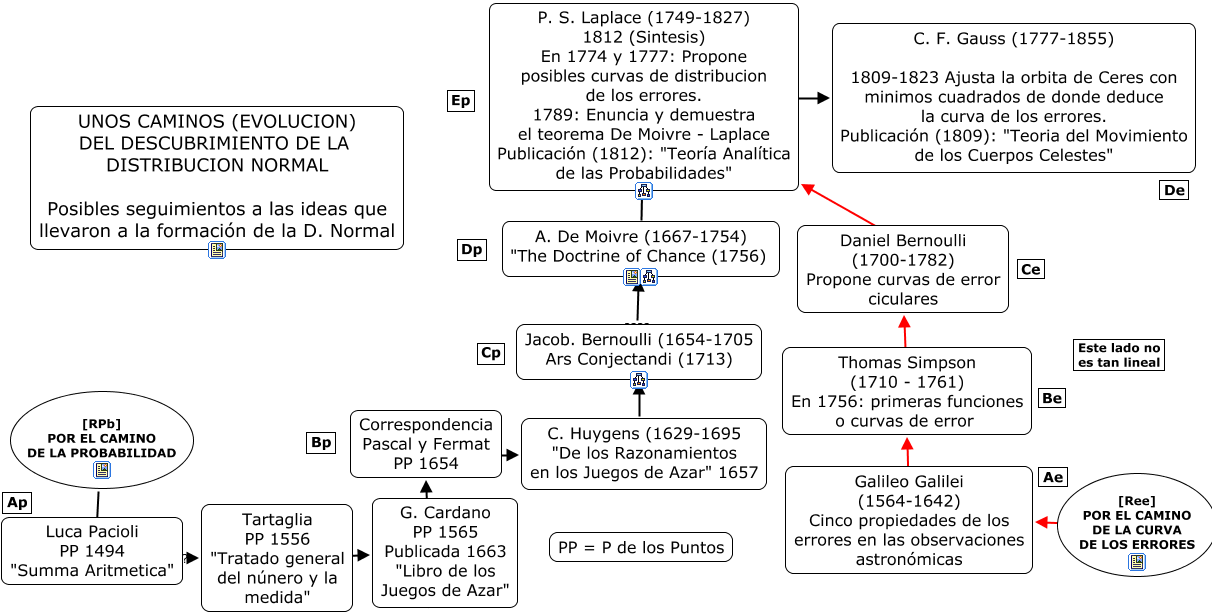
\includegraphics[scale=0.5,keepaspectratio=true]{./imagenes/dist-normal.png}
\caption{Dos posibles caminos del “descubrimiento” de la 	distribución normal. \citep{Conde2015}}
\label{fig2}
\end{figure*}

\subsection{Tablas}

  Las tablas, al igual que las figuras se deben incluir en el texto principal, cada tabla debe tener título y numeración con una descripción de la manera más breve pero más informativa posible. No deben utilizarse líneas verticales en la tabla y  los números deben ser alineados y uniformes en la cantidad de cifras decimales que presentan.
  
  Un buen ejemplo a seguir lo tenemos en la tabla \ref{tabla1}.
  
\begin{table}
\caption{Valores críticos de la distribución \textbf{DF}}
\label{tabla1}
\centering
\begin{tabular}{lccc}
\hline 
 & \multicolumn{3}{c}{\textbf{Nivel de significancia}} \\ 
\textbf{Distribución} & 10\% & 5\% & 1\% \\ 
\hline \hline
$\tau$ & -1.61 & -1.95 & -2.61 \\ 
$\tau$ intercepto & -3.51 & -2.89 & -2.58 \\  
$\tau$ int y tendencia & -3.15 & -3.45 & -4.04 \\  
$t$-student & -1.28 & -1.65 & -2.33 \\ 
\hline 
\end{tabular} 
\end{table}

Si la tabla es demasiado grande, de forma que debe ocupar las dos columnas se puede seguir el ejemplo de la tabla \ref{tabla2}. 

 \begin{table*}
	\caption{Comportamiento de los indicadores según escenarios de análisis. \citep{Rubiano2015}}\label{tabla2}
	\centering
	%\scalebox{0.8}{%@{\extracolsep{\fill}}
	\resizebox{\textwidth}{!}{  
	  \begin{tabular}{ccccccccc}
	    \hline
	    \multirow{2}{*}{\textbf{ESCENARIO}} & \multirow{2}{5cm}{\centering{\textbf{FACTOR O COMBINACIÓN DE FACTORES}}} & \textbf{Ep} & \multicolumn{2}{c}{\textbf{Te}} & \textbf{PP} & \textbf{VCP} & \textbf{Ahorros por Oferta} & \textbf{Sobrecosto}\\
	    \cline{3-9}
	    &  & \textbf{\%PI} & \textbf{Año} & \textbf{Semanas} & \textbf{\%PI} & \textbf{\%PI} & \textbf{\%PI} & \textbf{\%PI}\\
	    \hline \hline
	    ACTUAL & ACTUAL & 91.2 & 1.923 & 101 & 10.66 & 1.80 & 3.8 & 5.6\\	    
	    1 & A & 91.2 & 1.115 & 58 & 71.44 & 1.80 & 3.8 & 5.6\\	    
	    2 & B & 91.2 & 1.846 & 96 & 15.23 & -4.0 & 3.8 & -0.2\\	    
	    3 & C & 91.2 & 1.750 & 91 & 37.86 & 1.80 & 3.8 & 5.6\\	    
	    4 & A,B & 91.2 & 1.058 & 55 & 76.00 & -4.0 & 3.8 & -0.2\\	    
	    5 & A,C & 91.2 & 1.000 & 52 & 91.20 & 1.80 & 3.8 & 5.6\\	    
	    6 & B,C & 91.2 & 1.750 & 91 & 37.86 & 1.80 & 3.8 & 5.6\\
	    7 & A,B,C & 91.2 & 0.962 & 50 & 91.20 & -4.0 & 3.8 & -0.2\\
	    \hline
	  \end{tabular}
	}
    \end{table*} 
  
  \subsection{Ecuaciones}

  Las ecuaciones deben aparecer centradas en el texto principal y deben identificarse secuencialmente con números entre paréntesis ajustados en el margen derecho. Las ecuaciones deben ser lo más claras posibles y todos sus componentes y variables deben estar definidos en el cuerpo principal del articulo cuando se presentan por primera vez.

En las ecuación \ref{eq01} se tiene un ejemplo de una ecuación sencilla.

\begin{equation}
\label{eq01}
\Delta Z_t = \alpha \beta^{'} Z_{t-1}+\Gamma_1 \Delta Z_{t-1}+\hdots+ \Gamma_p \Delta Z_{t-p}+\varepsilon_t
\end{equation}

En la ecuación \ref{eq02} se aprecia una ecuación larga, acomodada para que no afecte el diseño general del texto.

\begin{equation}
\label{eq02}
\begin{array}{lll}
Z_t & = & \mu+\Pi Z_{t-1}+\Gamma_1 \Delta Z_{t-1}+\hdots+ \\
& & \Gamma_{K-1} \Delta Z_{t-K+1}+\Phi D_t+\varepsilon_t
\end{array}
\end{equation}

En la ecuación \ref{eq03} \citep{Rios2015} se puede apreciar una ecuación matricial, con el texto más pequeño de forma que no se salga de la margen del texto.

\begin{equation}
\label{eq03}
\begin{scriptsize}
\begin{bmatrix}
\Delta y_t\\
\Delta x_t
\end{bmatrix}
=
\begin{bmatrix}
\alpha_1\\
\alpha_2
\end{bmatrix}
\begin{bmatrix}
1-\beta
\end{bmatrix}
\begin{bmatrix}{l}
y_{t-1}\\
x_{t-1}
\end{bmatrix} 
+ 
\begin{bmatrix}
\gamma_{11} & \gamma_{21}\\
\gamma_{21} & \gamma_{22}
\end{bmatrix} 
\begin{bmatrix}
\Delta y_{t-1}\\
\Delta x_{t-1}
\end{bmatrix}
+
\begin{bmatrix}
\varepsilon_{1t}\\
\varepsilon_{2t}
\end{bmatrix}
\end{scriptsize}
\end{equation}
  
  \section{Identificación y formato de las Referencias Bibliográficas}
  
  Se debe usar el sistema \emph{apalike} tal y como se encuentra en este documento. Esto hace posible que la identificación de las referencias a lo largo del texto principal se realicen por el apellido del primer autor y el año de publicación entre paréntesis. Si un mismo autor tiene más de una publicación en el mismo año, deben distinguirse con letras a, b, c, etc. Por ejemplo: Prez (2003a). Si una referencia es de 3 autores o más, se utiliza la abreviatura et al. Por ejemplo, Ramírez et al. (2006).

  La lista de referencias debe estar ordenada alfabéticamente por el primer autor, teniendo el año como segundo criterio de ordenamiento. Debe existir una correspondencia uno a uno entre las referencias citadas en el articulo y las referencias listadas al final.
  
  \section{Conclusiones}

  Una sección de conclusiones es requerida. Aunque una conclusión puede repasar los puntos principales del documento, no debe repetir lo escrito en el resumen. Una conclusión podría extender la importancia del trabajo o podría hacer pensar en aplicaciones y extensiones futuras.
  
  \section{Apéndice}

  Esta sección es opcional.
  
  Para obtener más ayuda sobre la edición de textos académicos con LaTeX puede consultar \citep{Borbon2014}. 

  \section{Agradecimientos}

  Esta sección es opcional.


\bibliographystyle{apalike}
\bibliography{./plantilla}

  \label{UltimaPagina}
\end{document}